We ran OTM-MPI on Cori, a Cray XC40 supercomputer at NERSC~\cite{Cori}. Each of Cray's processing nodes has two sockets, each with a 16-core Intel\textcopyright~Xeon\texttrademark~Processor E5-2698 v3 (``Haswell'') at 2.3 GHz and 128 GB of RAM memory. This is a very modern parallel computer, taking advantage of recent advances in parallel computing technology. We report here two experiments; one with a model of Chattanooga, TN, and another with a large synthetic network. 

\subsection{Experiments with the Chattanooga network}

OTM includes a module for extracting networks from Open Street Maps \cite{otmtools,haklay2008openstreetmap}. This module was used to construct a model of  Chattanooga, Tennessee (see Figure~\ref{fig:chattanooga}). The goal of this experiment is to demonstrate the improvements in computation time that can be achieved by distributing computation over many processes for a realistic traffic network topology. Traffic performance metrics were not collected, nor was any effort made to reproduce the demand or routing characteristics of Chattanooga. The network has 32,260 nodes, 38,440 links, and contains 248 source links. Each of these was supplied with a large congestion-inducing demand of 2,000 vph per lane. We conducted 9 runs. In each, the number of parallel processes used was doubled, starting from a single process and up to 256 processes. Each trial was initialized with an empty network and was advanced 10,000 time steps. Figure \ref{fig:chattanooga_plots} shows the results of the simulation performance. 

\begin{figure}[!ht]
\centering
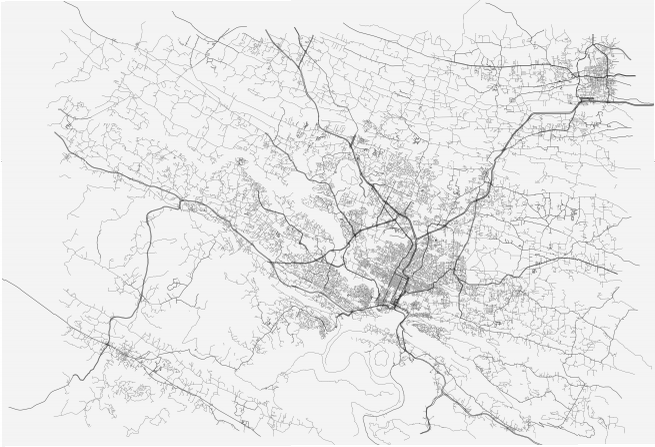
\includegraphics[width=\columnwidth]{figs/chattanooga.png}
\caption{OTM model of the Chattanooga, TN. Bounding box: 34.753\degree north, 35.445\degree south, -85.506\degree east, -84.902\degree west. This model has 32,260 nodes and 38,440 links. }
\label{fig:chattanooga}
\end{figure}

In all of the subplots of the figure, the x-axis is the number of processes involved in the simulation ($n$), represented in base-2 logarithmic scale. The first plot shows that, as expected, the average size of the subnetworks generated by METIS is inversely proportional to the number of processes. The second subplot shows the setup time of the program. This includes the network load time and the time taken to create the MPI communicator and distribute the message decoders. Notice that this load time reaches a minimum and increases slightly for 256 processes. This is because, although the subnetworks are smaller, the complexity of the metagraph and decoders increases and becomes significant for $n=256$. 
\begin{figure}[!ht]
\centering
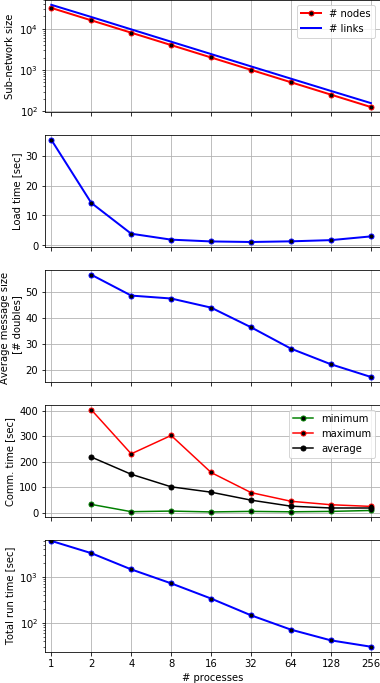
\includegraphics[width=\columnwidth]{figs/chattanooga_plots.png}
\caption{Simulation results for the Chattanooga network.}
\label{fig:chattanooga_plots}
\end{figure}

The third plot shows the average size of the messages being passed through the MPI communicator. For $n=2$, each process sends an average of 56 floats to each of its neighbors in the metagraph. As $n$ increases, the size of the messages gets smaller, while the number of messages and the total amount of information increases. The fourth subplot shows that the total time spent in communication generally \textit{decreases} with larger $n$. The graph communicator can more quickly transmit many small messages than a few large messages. This trend is true on average, however the plot also shows that the maximum and minimum communication times are not monotonic. 

Finally the fifth subplot shows the total run time, including load, communication, and computation time, on a log-log scale. The nearly linear trend indicates an inverse proportional relation between run time and the number of processes.  For this network, the execution on a single process took 6,026 seconds (1 hour and 40 minutes), and was reduced to 30.6 seconds when run with 256 cores. This corresponds to speedup  of 198.
 
\subsection{Experiment with a synthetic network}
\begin{figure}[!ht]
    \centering
    \includegraphics[height=0.5\columnwidth]{figs/Grid-Network.png}
    \caption{Topology of a synthetic network with 81,250 nodes and 268,000 links.}
    \label{fig:Synthetic_Network}
\end{figure}

We conducted experiments on a large, grid-like synthetic network, with a tiled topology as shown in Figure~\ref{fig:Synthetic_Network}. The goal of this experiment was to test the program on a second larger network, this one with 81,250 nodes and 268,000 links, which is about seven times the size of the Chattanooga network (in terms of links). 

Source flows were placed on 15,620 source links, again in sufficient amount to create congestion. The simulation was run with $n$ ranging from 1 to 1,024 processes (11 runs), and run for 1,000 simulated seconds each. 

\begin{figure}[!ht]
    \centering
    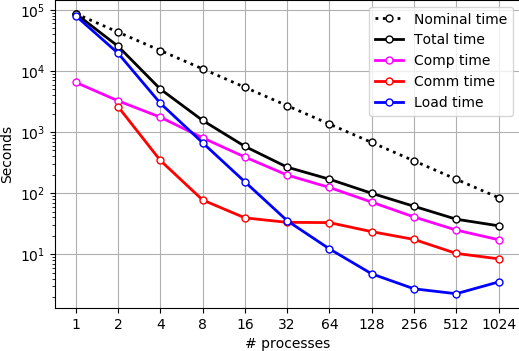
\includegraphics[width=\columnwidth]{figs/syntheticplot.png}
    \caption{Run times with the grid-like network.}
    \label{fig:mpirun}
\end{figure}


Figure \ref{fig:mpirun} shows the decomposition of the total simulation time into its three components: load time, communication time, and computation time. It also shows the `nominal' run time, which equals the serial total run time (with $n=1$) divided by the number of processes ($n$). This is the execution time that would be achieved if, for example, a simulation with 4 processes took one quarter of the time taken by the serial run. Such inversely proportional improvement is represented by a  straight line with negative unit slope in the log-log plot. Notice that the computation time indeed decreases at approximately this rate. However, the load time decreases at a rate that is approximately proportional to $1/n^2$ for $n\leq 32$. This is likely due to the large amount of memory required to store the network. The rate of improvement of the load time diminishes for $n \in[64, 512]$ and eventually worsens for $n>512$. This is due to the overhead involved in reading the network files. It can be seen then that the total simulation time is dominated by the load time for small values of $n$ ($n\leq 8$), which leads to super nominal (better than inversely proportional) improvements. For larger $n$ ($n\geq 16$), the total time is dominated by the computation time, which leads to inversely proportional improvements. For very large $n$ ($n\geq 512)$, the communication time begins to be significant, although it remains at about on tenth of the total simulation time for $n=1024$. The total simulation time was reduced by a factor of about 2,800 with $n=1024$, and could be further reduced with larger values. 

% The lower plot focuses on the simulations that are not distinguishable in the upper plot ($n\geq 6$). The trend is similar as in the first example, with inverse proportionality between the simulation time and the number of processes. 

% \begin{figure}[!ht]
%     \centering
%     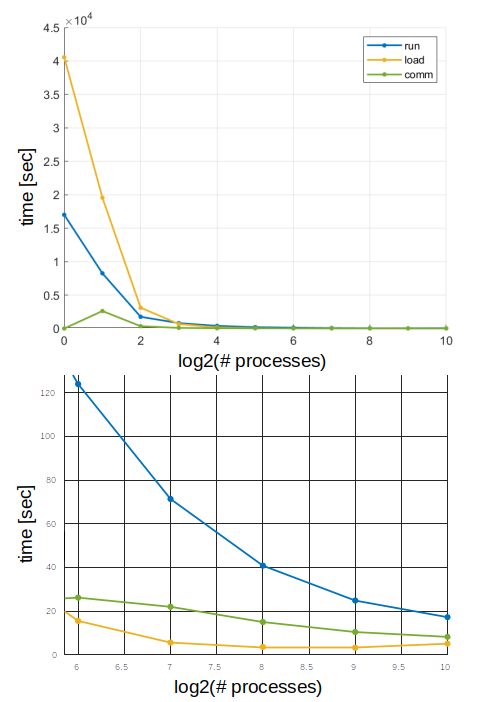
\includegraphics[width=\columnwidth]{figs/synthetic_results.png}
%     \caption{Parallel run times of the three phases of the algorithm with the grid-like network.}
%     \label{fig:mpirun}
% \end{figure}

% Figure~\ref{fig:scaling} demonstrate the scaling of OTM-MPI compared to the ideal scaling simulation rate. For each simulation experiment, the simulation rate $1/(simulation \:time)$, which corresponds to the number of simulations that can be completed within 1 seconds (simulations/s). The ideal rate is calculated as $(number\: of\: processes)*(serial\: simulation\: rate)$, and assumes that simulation rate increases proportionally with the number of processes. In practice, parallel simulation does not attain the ideal scaling rate as the $(communication\:time)/(simulation\:time)$ ratio grows with the number of processes. In fact, we observed that for the experiment with 1024 processes, each process spend half of its computation time in communicating with other processes. However, we still observed that for the simulation time, the parallel OTM had a speed up of 475 times with 1024 processes compared to the serial OTM. This corresponded to a time reduction from 8,245 seconds to 17 seconds.

% \begin{figure}[!ht]
%     \centering
%     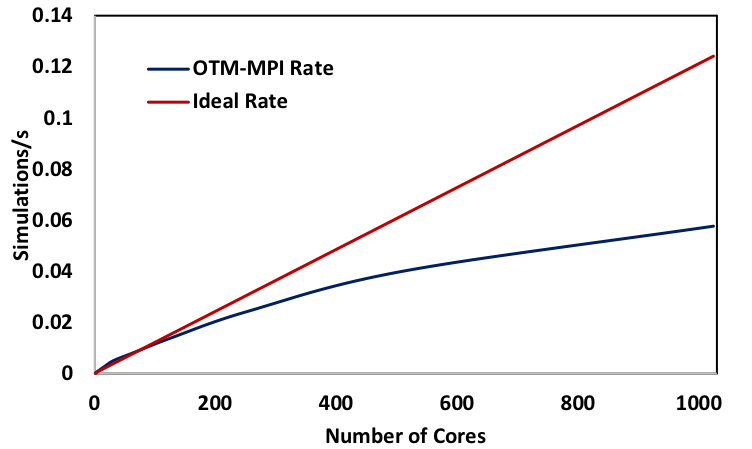
\includegraphics[width=\columnwidth]{figs/Scaling.png}
%     \caption{OTM scaling  compared to ideal scaling for the grid network.}
%     \label{fig:scaling}
% \end{figure}

